\section{Introduction to Distributed Systems}

%##################################################
\subsection{Definition of a Distributed System}
%##################################################

A distributed system is a \ac{CN} providing some kind of abstraction/transparency provided by the transport layer and potentially by some kind of middleware. Distributed systems are looked at from the application layer of the TCP/IP model.

%##################################################
\subsection{Challenges}
%##################################################

There are three basic challenges, which together form the \textit{bermuda triangle} of distributed systems:

\begin{enumerate}
    \item \textbf{No accessible global state:} The individual nodes might be in any state, which cannot be known at all other nodes at all times.
    \item \textbf{No common time/clock:} As every system has its own clock and the transmission of messages requires time, the clocks of nodes cannot be synchronized perfectly.
    \item \textbf{Indeterminism:} Due to race conditions and erroneous networks, the program execution for the whole system is non-deterministic.
\end{enumerate}

%##################################################
\subsection{Requirements}
%##################################################

We would like to require distributed systems to have certain properties. These properties differ from book to book, but we will define the following seven properties for this lecture:

\begin{enumerate}
    \item \textbf{Heterogeneity Support:} Different hardware, operating systems and programming languages are supported.
    \item \textbf{Openness:} Anyone might participate! Therefore open known standard protocols shall be used.
    \item \textbf{Scalability:} Scalability concerning processors, memory, storage, and nodes.
    \item \textbf{Security:} Secure the network, because malicious users may try to compromise it.
    \item \textbf{Fault Tolerance:} We would like to be resilient to node (\ac{AS}) and network (\ac{CSS}) failures.
    \item \textbf{Concurrency:} Distributed Networks are inherently concurrent. We of course want to take advantage of this property. However, then we need to ensure consistency e.g. when concurrently accessing shared resources.
    \item \textbf{Transparency:} We would like to abstract from different properties of the \ac{CN}
\end{enumerate}

%##################################################
\subsection{Abstraction Levels}
%##################################################

There are several abstraction layers, from which we can look at distributed systems. In the following, we divide into 4 levels, which are ordered ascending by their level of abstraction. When talking about distributed systems, we would like to be at level 3 or 4.

\begin{enumerate}
    \item \textbf{Physical configuration:} How are nodes connected physically i.e. using which typology and which transmission channels.
    \item \textbf{Logical configuration:} Looking at the network from the \textit{transport layer}.
    \item \textbf{Process network:} Processes communicate using messages. The real location of the processes in the computer network is hidden. This is the abstraction layer of e.g. MPI.
    \item \textbf{Distributed Algorithm:} This abstraction layer defines distributed algorithms regardless of the target environment, the target configuration (e.g. number of processors and RAM) and the programming language.
\end{enumerate}

%##################################################
\subsection{Transparency}
%##################################################

We would like distributed systems to provide transparency concerning certain properties. Transparency here means the concealment of the property. The properties are:

\begin{enumerate}
    \item \textbf{Access:} The interface for accessing resources is identical regardless of the node, which is accessed.
    \item \textbf{Location:} Resources are accessed without knowledge about their physical/network-level location.
    \item \textbf{Concurrency:} Several processes act concurrently on shared resources, but the user experiences simulated single-user execution.
    \item \textbf{Replication:} Multiple instances of e.g. compute nodes or data are used for performance or reliability reasons without the user noticing this.
    \item \textbf{Failure:} Node and network failures are concealed.
    \item \textbf{Mobility:} Resources might change their physical location during program execution without the user noticing it.
    \item \textbf{Performance:} Local and remote accesses happen with similar performance. In practice, this is often not the case.
    \item \textbf{Scaling:} Allows scalability without changes to the system structure or the user-defined algorithms.
\end{enumerate}

%##################################################
\subsection{Classification}
%##################################################

According to Flynn's taxonomy, distributed systems can be classified as the \ac{MIMD} model.

Furthermore, they can be classified based on their distributed property. In practice, usually more than one property is distributed:

\begin{enumerate}
    \item \textbf{Function Federation:} The systems functionality is distributed over nodes.
    \item \textbf{Load Federation:} Balancing load using multiple nodes.
    \item \textbf{Data federation:} Distributing data on different nodes.
    \item \textbf{Availability:} Increasing Availability through replication.
\end{enumerate}

%##################################################
\subsection{Tier Architectures}
%##################################################

Applications can be distributed into multiple layers, which then result in Tier-architectures:

\begin{enumerate}
    \item \textbf{2-Tier:} \ac{GUI} on one tier, DBMS on other tier.
    \item \textbf{3-Tier:} Client \textendash{} Application Server \textendash{} Database Server
    \item \textbf{n-Tier:} Splitting the application further into $n$ tiers, where each tier might consist of several nodes.
\end{enumerate}

%##################################################
\subsection{Fundamental Approaches}
%##################################################

There are 4 fundamental approaches for writing distributed software. The most widespread approach, which is also a topic of this lecture, is the distributed programming approach:

\begin{enumerate}
    \item \textbf{Distributed Operating System:} This approach constructs an entire \ac{OS} built on top of a computer network, such that parallel programming and distributed storage are already supported by the \ac{OS}. However, because this approach is too overkill for specific use cases, where distribution is not required, it never became widespread. Today, the network \ac{OS}, which adds network integration on \ac{OS}-level (e.g. Mounting cloud storage, online authorization), is more common.
    \item \textbf{Distributed Database:} Distributed databases allow for scalable and accessible storage of data. However, they do not provide much infrastructure when writing parallel algorithms. Distributed databases exist e.g. as cloud storage, but have never reached internet scale, such that any computer could be used to retrieve any data.
    \item \textbf{Protocol Approach:} In this approach we define open protocols for communication to build distributed systems. This ensures openness and simplicity. On the counter side, only very limited functionality is supported and the distribution is usually only a client-server separation.
    \item \textbf{Distributed Programming:} This approach can be structured into 3 possible models:
          \begin{itemize}
              \item[$0$] The zero-support approach builds distributed programs on top of the transport layer using UDP or TCP directly.
              \item[\textbf{M}] The middleware approach uses a middleware to abstract from the transport layer. This is today's approach.
              \item[\textbf{D}] The distributed runtime system approach uses a parallel programming language and a distributed runtime. This results in compiler support for distributed programming. However, this is hard to realize and has seen no acceptance in the past 50 years. Maybe it could be the way to go in the future.
          \end{itemize}
\end{enumerate}

%##################################################
\subsection{System Models}
%##################################################

Distributed Systems can be classified based on their system model:

\begin{enumerate}
    \item \textbf{Client-Server:} The server is a fixed system participant, which provides functionality to clients.
    \item \textbf{Peer-2-Peer:} All nodes have the same functionality.
\end{enumerate}

%##################################################
\subsection{Distributed Programming Paradigms}
%##################################################

In figure \ref{fig:programming_paradigms} we see a taxonomy for distributed programming paradigms. We can structure them into pull- and push-paradigms.

\begin{figure}[h]
    \centering
    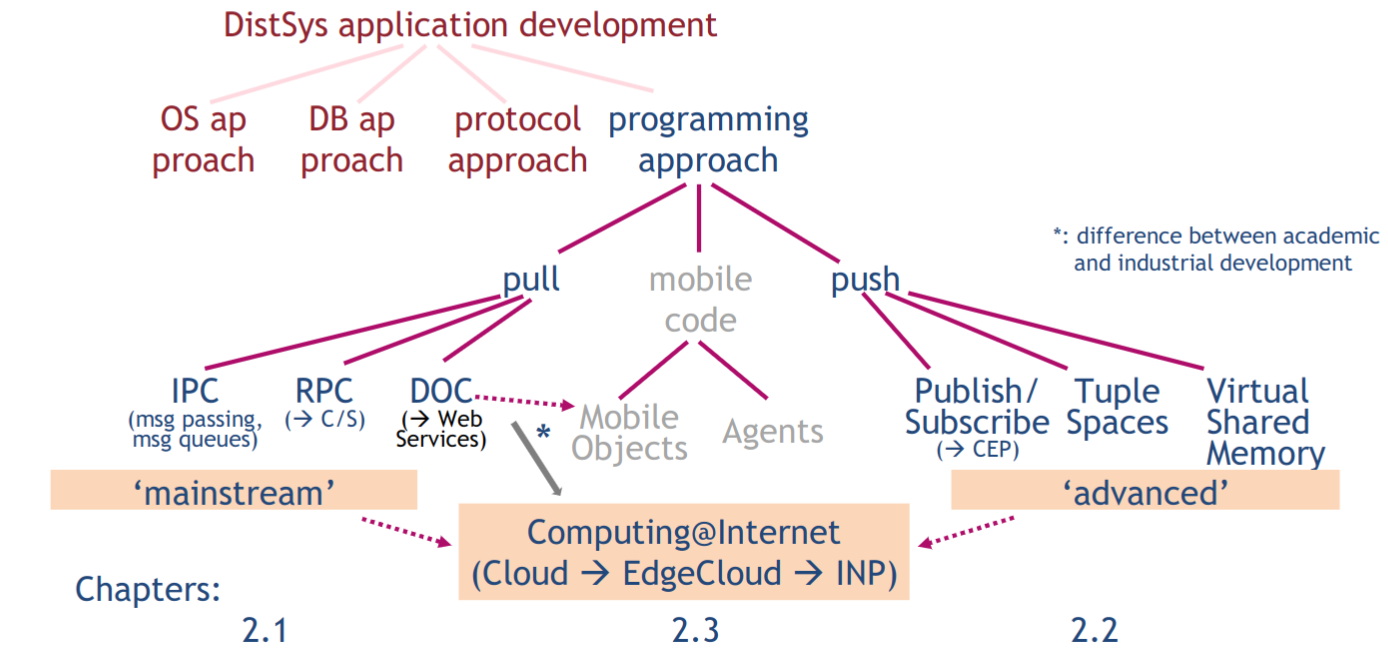
\includegraphics[width=\textwidth]{gfx/programming_paradigms.png}
    \caption{Pragmatic taxonomy of distributed programming paradigms}
    \label{fig:programming_paradigms}
\end{figure}
